\chapter{Исследование LQE/фильтра Калмана}
\label{ch:chap2}
\section{Условие задачи}

Рассмотреть систему:
$$
  \begin{cases}
    \dot{x} = Ax + Bu + f \\
    y = Cx + \xi
  \end{cases}
$$ и в нашем случае $(f, \xi)$ - гауссовский белый шум, выполнить следующие шаги:

\begin{itemize}
    \item  Проверить систему на обнаруживаемость.
    \item Построить схему моделирования системы с наблюдателем состояния $\dot{\hat{x}} = A \hat{x} + L(C\hat{x}-y)$
    \item Задаться подходящими значениями матриц $Q^* \succeq 0$ и $R^* \succ 0$ и 
значением параметра $\alpha > 0$ и сформировать четыре набора пар матриц $(Q,R)$:
\begin{itemize}
  \item $(Q,R);$
  \item $(\alpha Q,R);$
  \item $(Q, \alpha R);$
  \item $( \alpha Q, \alpha R);$
\end{itemize}
\item Для каждой из пар значений матриц $(Q,R)$ синтезировать наблюдатель, минимизирующий «критерий доверия».
\begin{itemize}
  \item Найти соответствующую матрицу наблюдателя $L$, обеспечивающую минимизацию функционала качества.
  \item Выполнить компьютерное моделирование.
\end{itemize}
\item Сравнить полученные результаты для различных пар $(Q,R)$, сделать выводы.

\end{itemize}
    
\newpage
\section{Решение задачи}

Параметры для объекта:
$$
  A = \begin{bmatrix}
    -35 & 11 & 6 & 11 \\
    -56 & 17 & 10 & 18 \\
    -22 & 7 & 5 & 6 \\
    -42 & 12 & 10 & 13 \\
\end{bmatrix} \tab
  C = \begin{bmatrix}
    -1 & 0 & 0 & 1 \\
\end{bmatrix}
$$

\subsection{Исследование наблюдаемости}
Найдём собственные числа матрицы $A$:
$$
    \sigma(A) = \{ \pm 3i, \pm 1i \}
$$
Воспользуемся критерием Калмана, система окажется полностью наблюдаемой:
$$
  rank(V) = rank(\begin{bmatrix}
    -1 & 0 & 0 & 1 \\
    -7 & 1 & 4 & 2 \\
    17 & -8 & 8 & -9 \\
    55 & -1 & -28 & -26 \\
\end{bmatrix}) = 4 = n
$$

Построим схему:

\begin{figure}[ht]
  \centering
  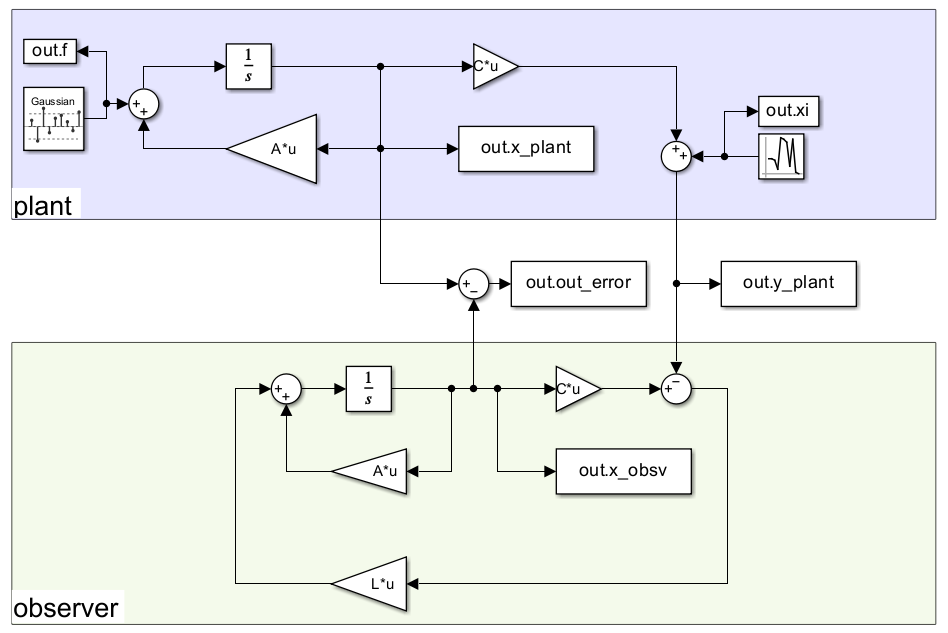
\includegraphics[width=0.8\textwidth]{model_observer_noise.png}
  \caption{Модель с фильтром калмана}
\end{figure}

В качестве случайных сигналов $f(t), \xi(t)$ возьмём диспресии у шумов:
$$
  \sigma(f) = 4,\tab \sigma(\xi) = 7
$$

Зададимся значениями матриц и параметра, на основе их сформируем четыре набора пар матриц $(Q,R)$:
$$
  \alpha = 15, \tab Q = \begin{bmatrix}
                        2 & 0 & 0 & 0\\
                        0 & 2 & 0 & 0\\
                        0 & 0 & 2 & 0\\
                        0 & 0 & 0 & 2
                      \end{bmatrix}, \tab R=4
$$


\subsection{Первый набор}
$$
  Q = \begin{bmatrix}
                    2 & 0 & 0 & 0\\
                    0 & 2 & 0 & 0\\
                    0 & 0 & 2 & 0\\
                    0 & 0 & 0 & 2
                      \end{bmatrix}, \tab R=4
$$

Синтезируем регулятор, минимизирующий функционал критерий доверия:
$$
  J = \int_{0}^{\infty} (f^T(t)Q^{-1} f(t) + \xi^T(t) R^{-1} \xi(t))dt  
$$
путем решения матричного уравнения Риккати при $\nu = 1$:
$$
    AP + PA^T + Q - \nu PC^T R^{-1} C P = 0, \tab L = -PC^T R^{-1}
$$
Положительно определённую матрицу $P$ мы сможем получить при выполнении следующих условий:
\begin{itemize}
  \item $Q \succeq 0$, $R \succ 0$
  \item $(C,A)$ - обнаруживаемая пара
  \item $(A, Q)$ - управляемая пара
\end{itemize}
Получим следующую матрицу коррекции $L$, обеспечивающую минимизацию функционала качества:
$$
   L = \begin{bmatrix}
    -9.28 \\
    -14.98 \\
    -7.54 \\
    -12.86 \\
\end{bmatrix}
$$

Выполним компьютерное моделирование замкнутой системы:

\begin{figure}[ht]
  \centering
  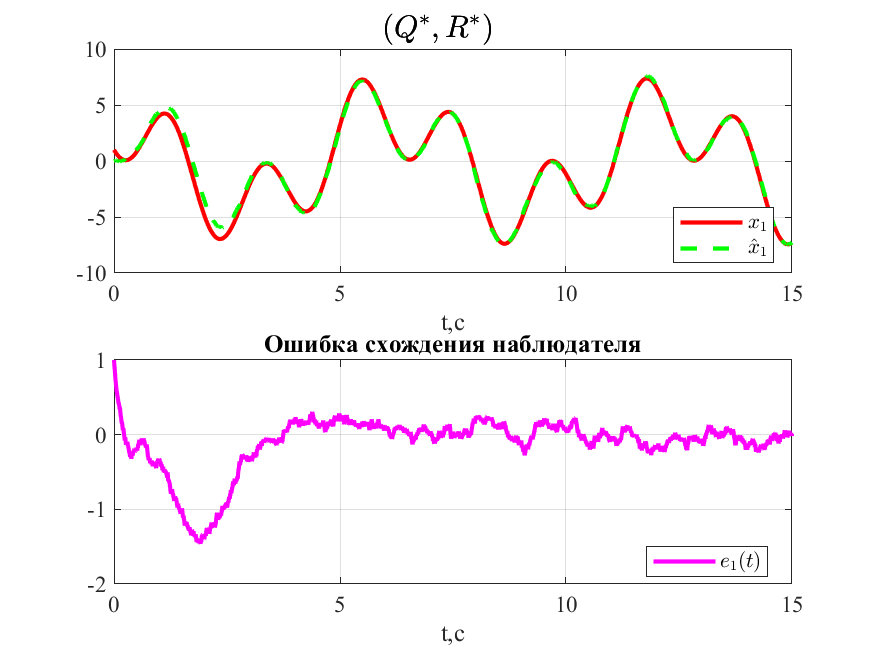
\includegraphics[width=0.8\textwidth]{obsv1.png}
  \caption{Состояние системы и фильтр Калмана}
\end{figure}
\newpage
\begin{figure}[ht]
  \centering
  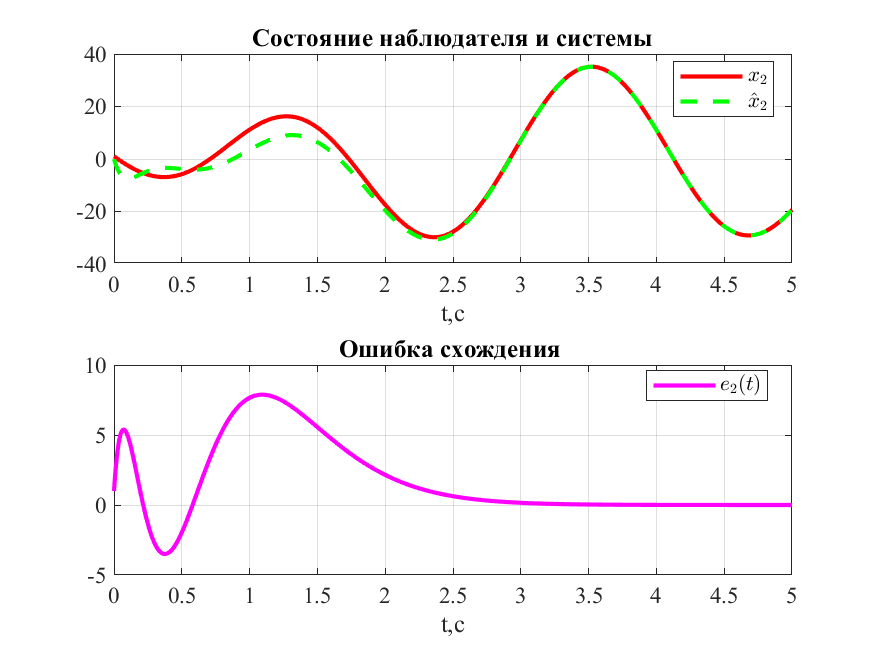
\includegraphics[width=0.8\textwidth]{obsv2.png}
  \caption{Состояние системы и фильтр Калмана}
\end{figure}
\newpage
\begin{figure}[ht]
  \centering
  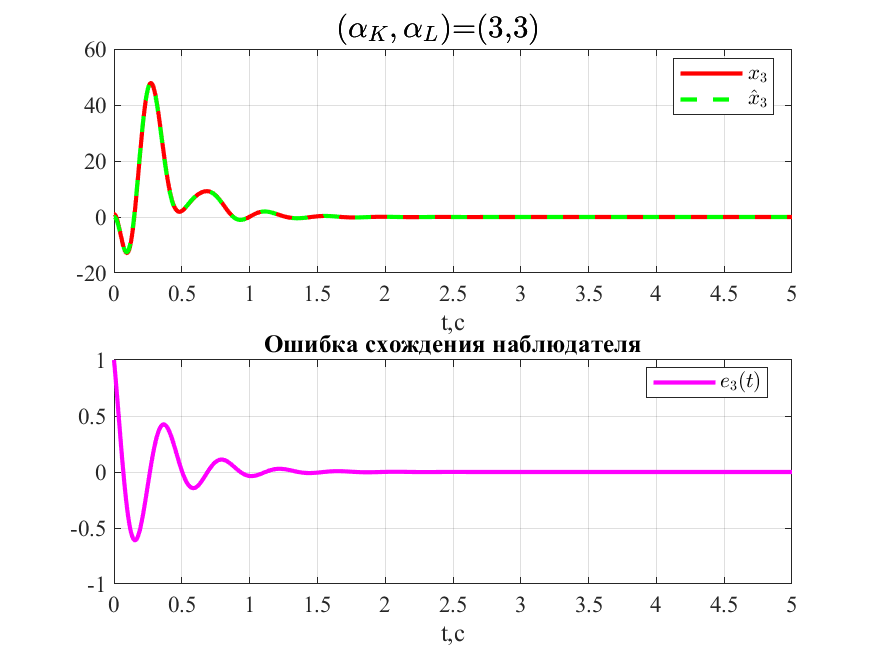
\includegraphics[width=0.8\textwidth]{obsv3.png}
  \caption{Состояние системы и фильтр Калмана}
\end{figure}
\begin{figure}[ht]
  \centering
  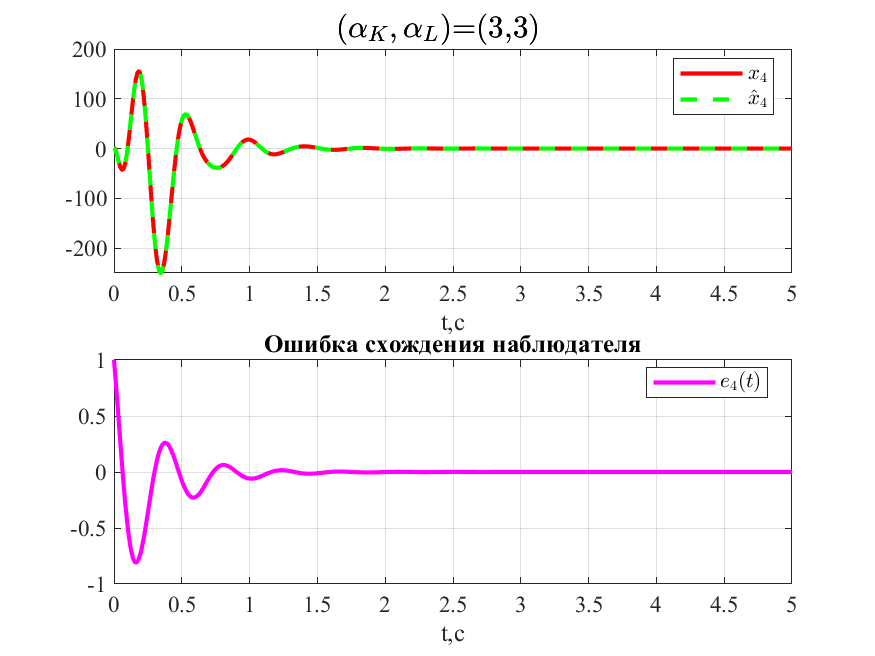
\includegraphics[width=0.8\textwidth]{obsv4.png}
  \caption{Состояние системы и фильтр Калмана}
\end{figure}


\subsection{Второй набор}
$$
  Q = \begin{bmatrix}
                    30 & 0 & 0 & 0\\
                    0 & 30 & 0 & 0\\
                    0 & 0 & 30 & 0\\
                    0 & 0 & 0 & 30
                      \end{bmatrix}, \tab R=4
$$

Аналогично прошлым пунктам, получим следующую матрицу коррекции $L$, обеспечивающую минимизацию функционала качества:
$$
   L = \begin{bmatrix}
    -16.53 \\
    -27.11 \\
    -17.35 \\
    -25.37 \\
\end{bmatrix}
$$


\begin{figure}[ht]
  \centering
  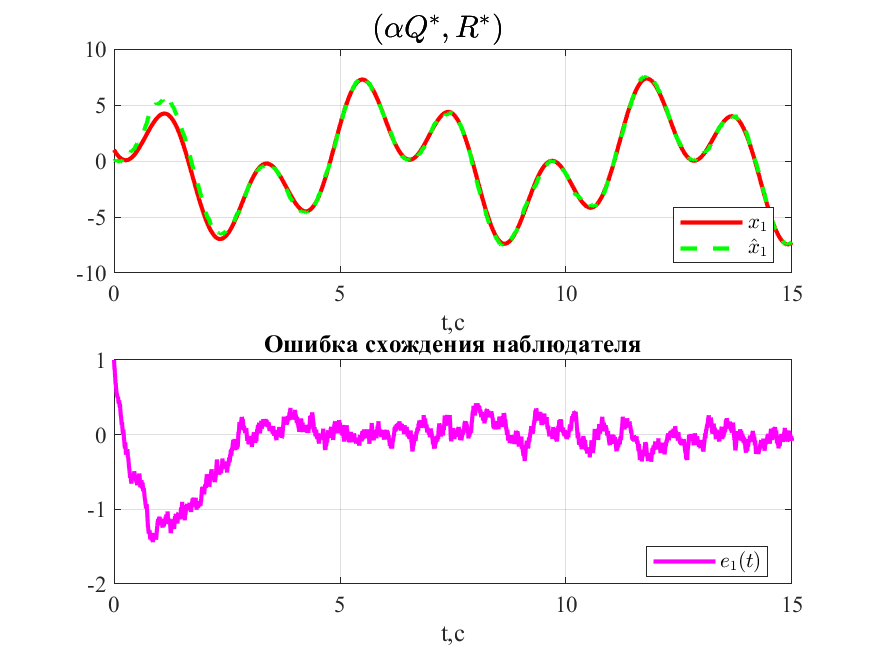
\includegraphics[width=0.8\textwidth]{obsv5.png}
  \caption{Состояние системы и фильтр Калмана}
\end{figure}
\newpage
\begin{figure}[ht]
  \centering
  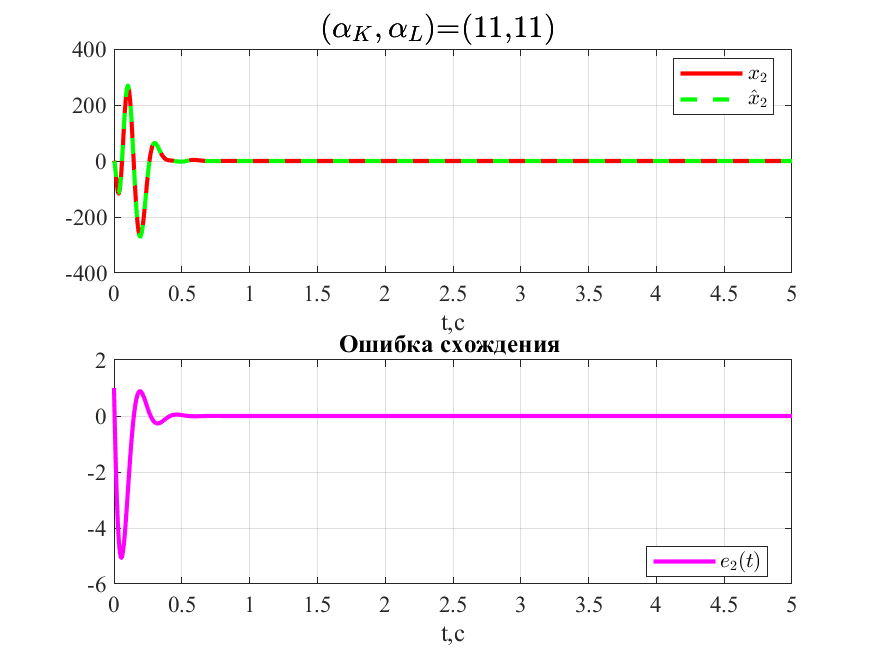
\includegraphics[width=0.8\textwidth]{obsv6.png}
  \caption{Состояние системы и фильтр Калмана}
\end{figure}
\begin{figure}[ht]
  \centering
  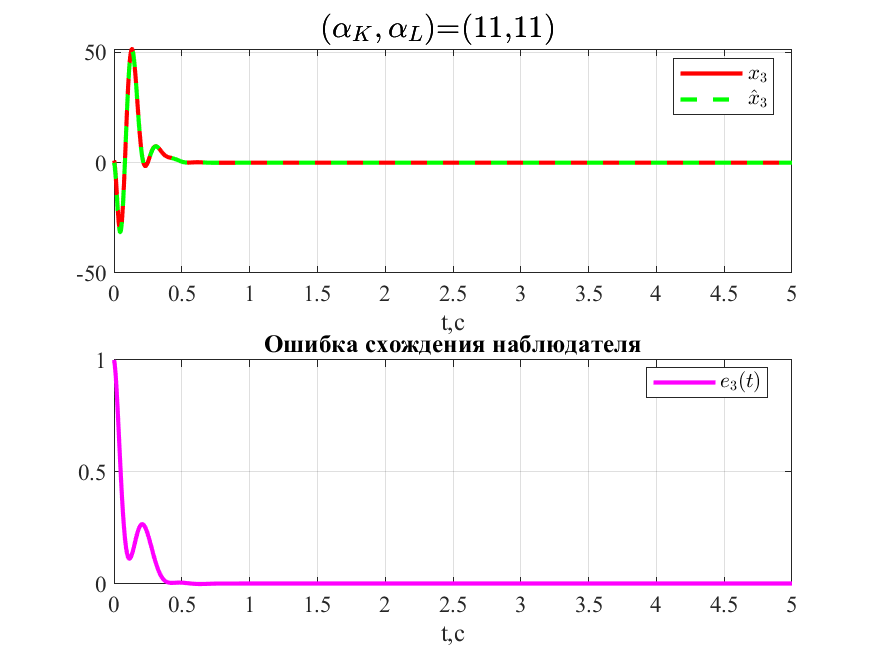
\includegraphics[width=0.8\textwidth]{obsv7.png}
  \caption{Состояние системы и фильтр Калмана}
\end{figure}
\newpage
\begin{figure}[ht]
  \centering
  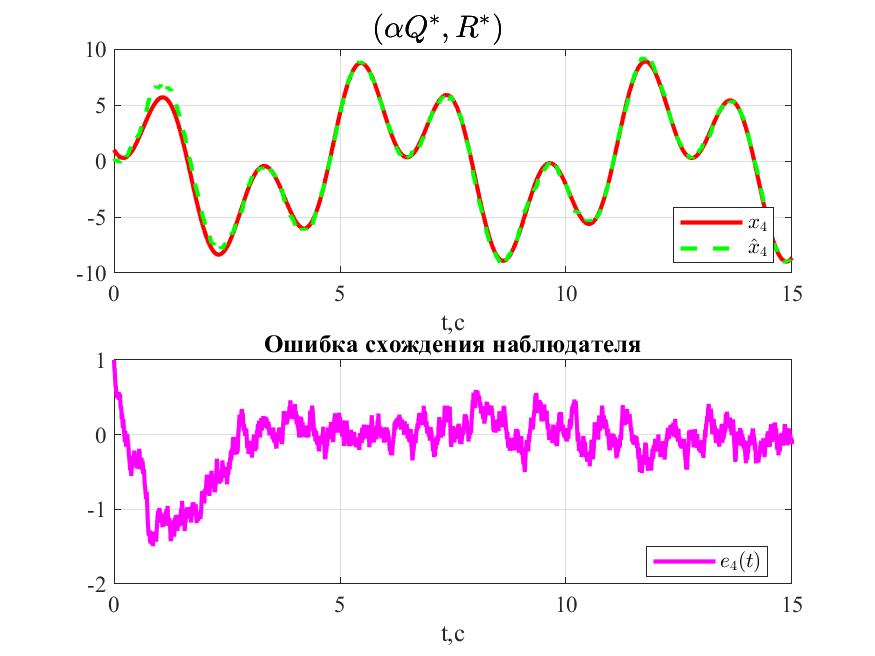
\includegraphics[width=0.8\textwidth]{obsv8.png}
  \caption{Состояние системы и фильтр Калмана}
\end{figure}


\subsection{Третий набор}
$$
  Q = \begin{bmatrix}
                    2 & 0 & 0 & 0\\
                    0 & 2 & 0 & 0\\
                    0 & 0 & 2 & 0\\
                    0 & 0 & 0 & 2
                      \end{bmatrix}, \tab R=60
$$

Аналогично прошлым пунктам, получим следующую матрицу коррекции $L$, обеспечивающую минимизацию функционала качества:
$$
   L = \begin{bmatrix}
    -3.49 \\
    -5.57 \\
    -2.56 \\
    -4.6 \\
\end{bmatrix}
$$


\begin{figure}[ht]
  \centering
  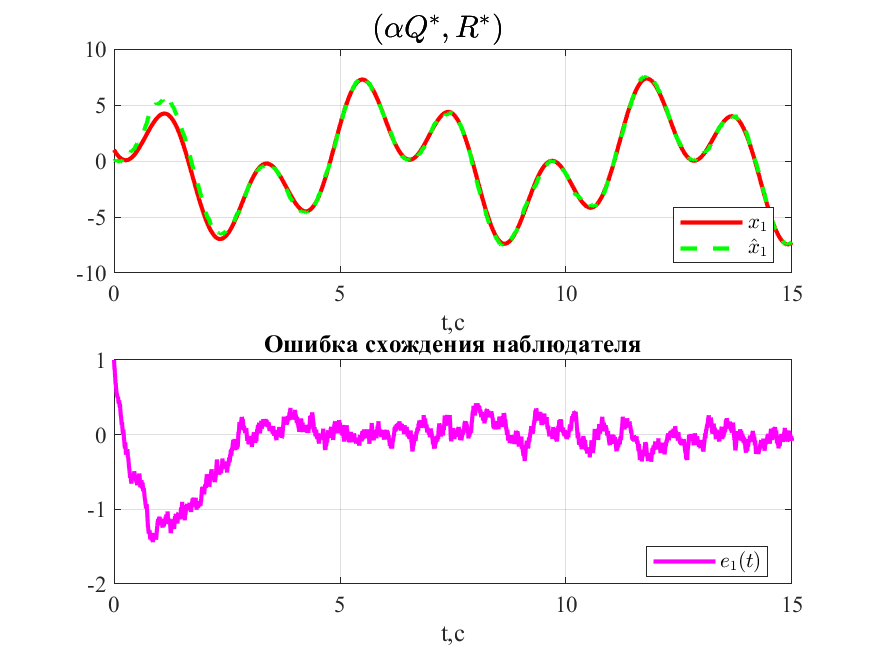
\includegraphics[width=0.8\textwidth]{obsv5.png}
  \caption{Состояние системы и фильтр Калмана}
\end{figure}
\newpage
\begin{figure}[ht]
  \centering
  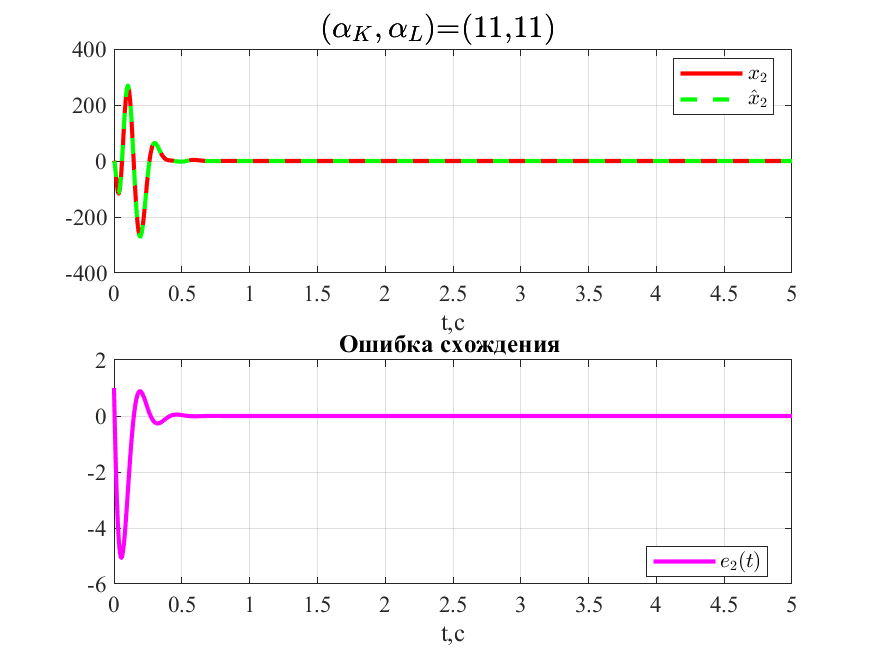
\includegraphics[width=0.8\textwidth]{obsv6.png}
  \caption{Состояние системы и фильтр Калмана}
\end{figure}
\begin{figure}[ht]
  \centering
  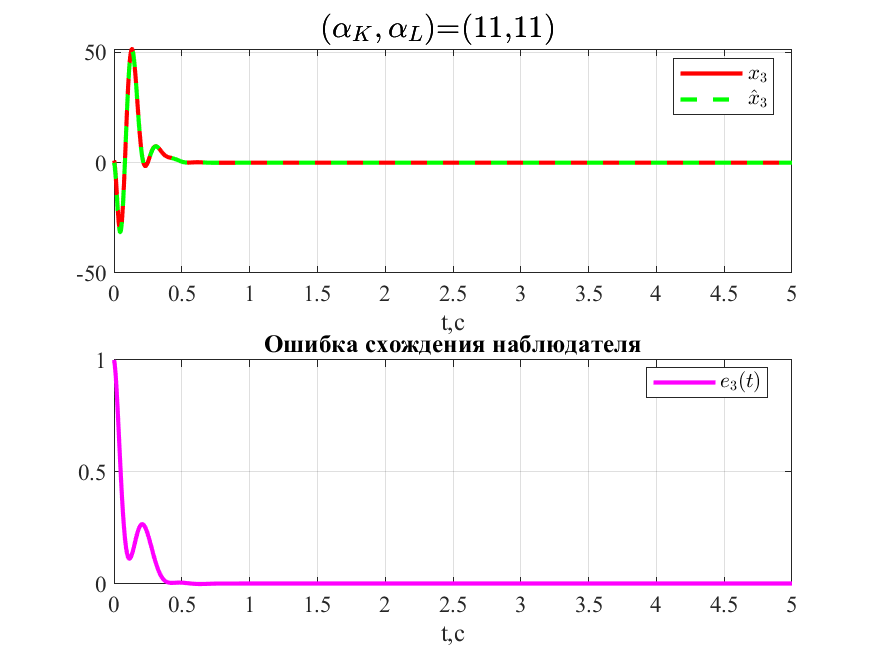
\includegraphics[width=0.8\textwidth]{obsv7.png}
  \caption{Состояние системы и фильтр Калмана}
\end{figure}
\newpage
\begin{figure}[ht]
  \centering
  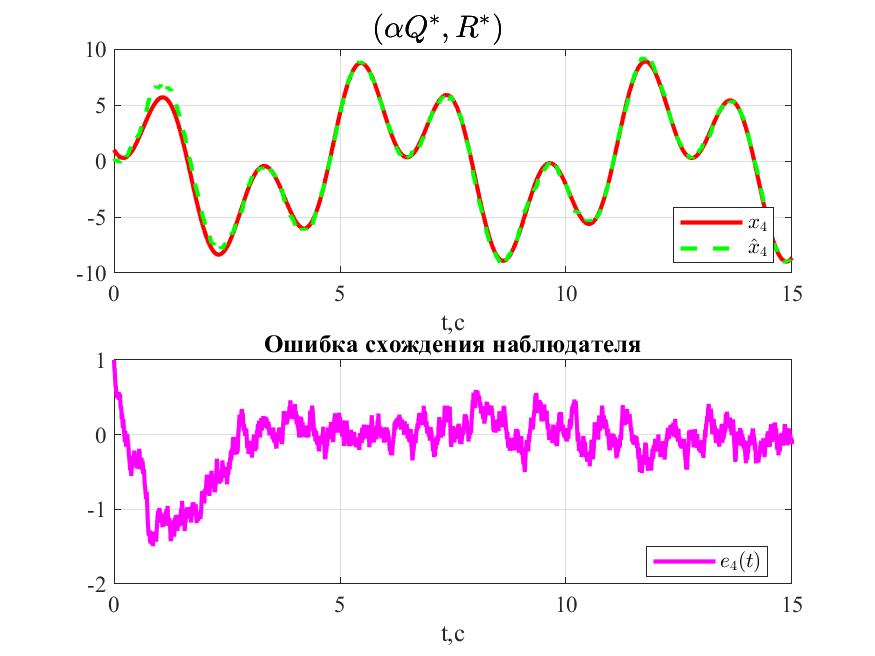
\includegraphics[width=0.8\textwidth]{obsv8.png}
  \caption{Состояние системы и фильтр Калмана}
\end{figure}

\subsection{Четвертый набор}
$$
  Q = \begin{bmatrix}
                      30 & 0 & 0 & 0\\
                      0 & 30 & 0 & 0\\
                      0 & 0 & 30 & 0\\
                      0 & 0 & 0 & 30
                      \end{bmatrix}, \tab R=60
$$

Аналогично прошлым пунктам, получим следующую матрицу коррекции $L$, обеспечивающую минимизацию функционала качества:
$$
   L = \begin{bmatrix}
    -9.28 \\
    -14.98 \\
    -7.54 \\
    -12.86 \\
\end{bmatrix}
$$

\begin{figure}[ht]
  \centering
  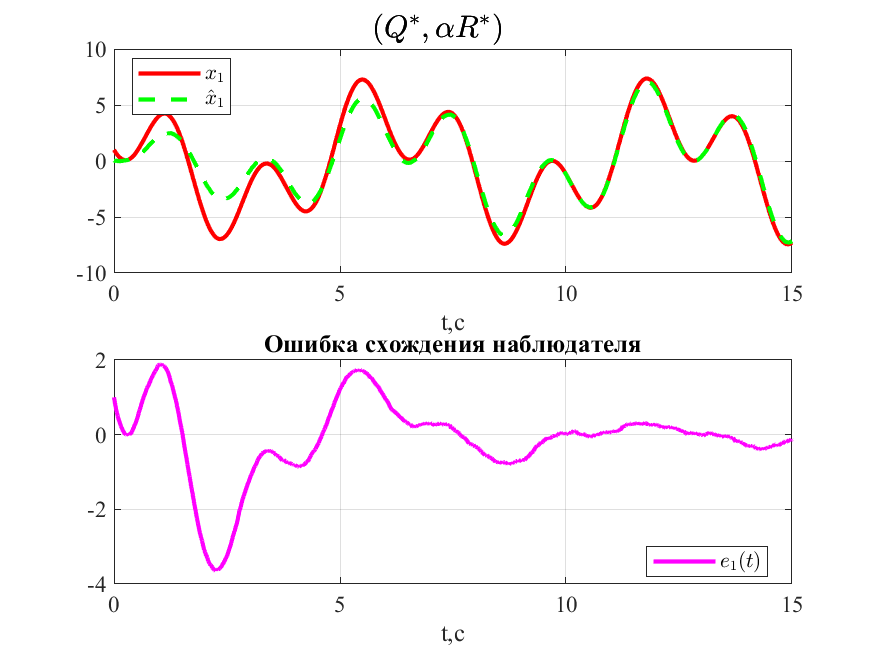
\includegraphics[width=0.8\textwidth]{obsv9.png}
  \caption{Состояние системы и фильтр Калмана}
\end{figure}
\newpage
\begin{figure}[ht]
  \centering
  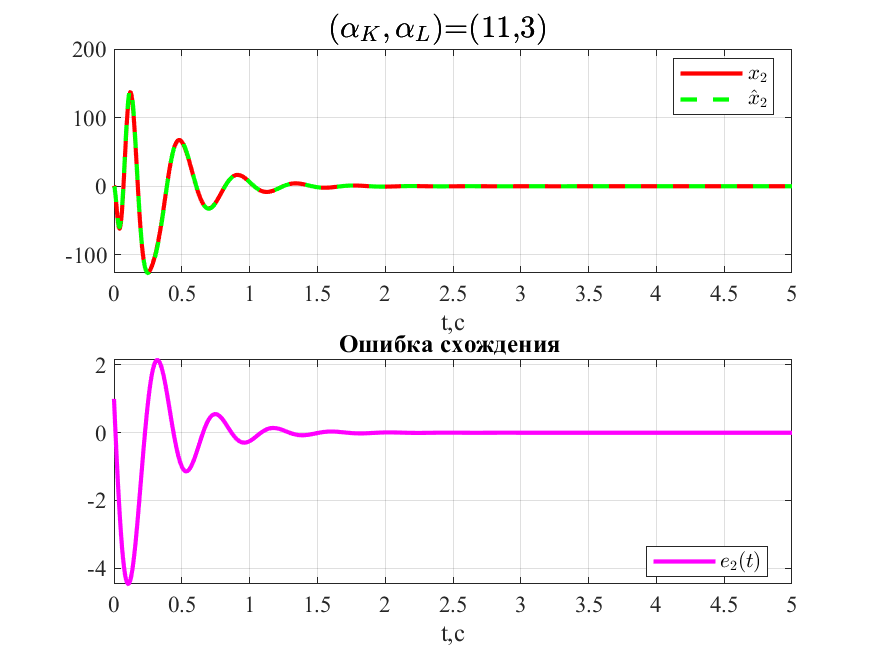
\includegraphics[width=0.8\textwidth]{obsv10.png}
  \caption{Состояние системы и фильтр Калмана}
\end{figure}
\begin{figure}[ht]
  \centering
  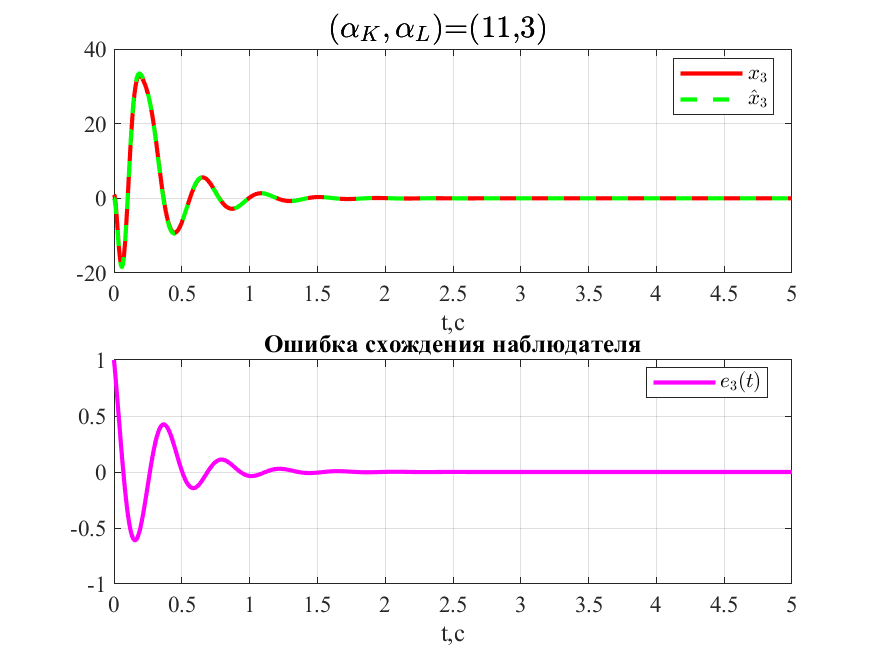
\includegraphics[width=0.8\textwidth]{obsv11.png}
  \caption{Состояние системы и фильтр Калмана}
\end{figure}
\newpage
\begin{figure}[ht]
  \centering
  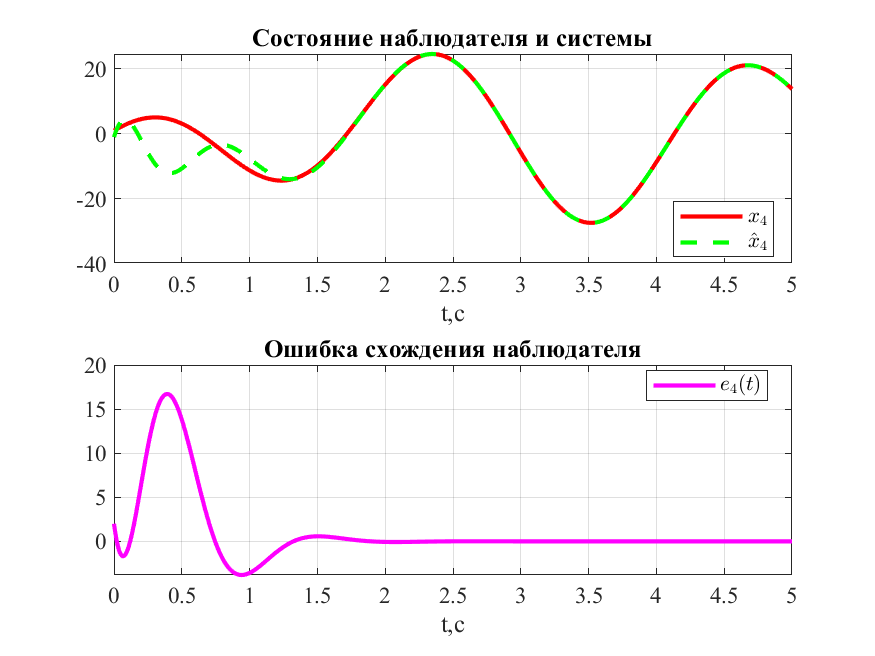
\includegraphics[width=0.8\textwidth]{obsv12.png}
  \caption{Состояние системы и фильтр Калмана}
\end{figure}

Как можно заметить - 1, 2, 4 подобранная пара параметров не позволяют качественно отфильтровать наблюдателю сигнал, 
поэтому на выходе мы получили некоторую шумную ошибку около нуля. Но при большом недоверии к "шумных датчикам", фильтр калмана уже качественно подавляет шум у ошибки.

\subsection{Вывод}
В этом задании мы синтезировали фильтр Калмана для задачи наблюдения за системой, устойчивой по Ляпунову, с добавлением внешних возмущений и шума на выходе в виде белого шума.
С ними мы боролись при помощи фильтра, которому мы задавали
\endinput 